% ========================================
%	Header einbinden
% ========================================

\documentclass[bibtotoc,titlepage]{scrartcl}

% Deutsche Spracheinstellungen
\usepackage[ngerman,german]{babel, varioref}
\usepackage[T1]{fontenc}
\usepackage[utf8]{inputenc}

%\usepackage{marvosym}

\usepackage{amsfonts}
\usepackage{amssymb}
\usepackage{amsmath}
\usepackage{amscd}
\usepackage{amstext}

\usepackage{longtable}

%\usepackage{bibgerm}

\usepackage{footnpag}

\usepackage{ifthen}                 %%% package for conditionals in TeX
\usepackage[amssymb]{SIunits}
%Für textumflossene Bilder und Tablellen
%\usepackage{floatflt} - veraltet

%Für Testzwecke aktivieren, zeigt labels und refs im Text an.
%\usepackage{showkeys}

% Abstand zwischen zwei Absätzen nach DIN (1,5 Zeilen)
% \setlength{\parskip}{1.5ex plus0.5ex minus0.5ex}

% Einrückung am Anfang eines neuen Absatzes nach DIN (keine)
%\setlength{\parindent}{0pt}

% Ränder definieren
% \setlength{\oddsidemargin}{0.3cm}
% \setlength{\textwidth}{15.6cm}

% bessere Bildunterschriften
%\usepackage[center]{caption2}


% Problemlösungen beim Umgang mit Gleitumgebungen
\usepackage{float}

% Nummeriert bis zur Strukturstufe 3 (also <section>, <subsection> und <subsubsection>)
%\setcounter{secnumdepth}{3}

% Führt das Inhaltsverzeichnis bis zur Strukturstufe 3
%\setcounter{tocdepth}{3}
\usepackage[version=3]{mhchem}
	\mhchemoptions{minus-sidebearing-left=0.06em, minus-sidebearing-right=0.11em}
\usepackage{exscale}

\newenvironment{dsm} {\begin{displaymath}} {\end{displaymath}}
\newenvironment{vars} {\begin{center}\scriptsize} {\normalsize \end{center}}


\newcommand {\en} {\varepsilon_0}               % Epsilon-Null aus der Elektrodynamik
\newcommand {\lap} {\; \mathbf{\Delta}}         % Laplace-Operator
\newcommand {\R} { \mathbb{R} }                 % Menge der reellen Zahlen
\newcommand {\e} { \ \mathbf{e} }               % Eulersche Zahl
\renewcommand {\i} { \mathbf{i} }               % komplexe Zahl i
\newcommand {\N} { \mathbb{N} }                 % Menge der nat. Zahlen
\newcommand {\C} { \mathbb{C} }                 % Menge der kompl. Zahlen
\newcommand {\Z} { \mathbb{Z} }                 % Menge der kompl. Zahlen
\newcommand {\limi}[1]{\lim_{#1 \rightarrow \infty}} % Limes unendlich
\newcommand {\sumi}[1]{\sum_{#1=0}^\infty}
\newcommand {\rot} {\; \mathrm{rot} \,}         % Rotation
\newcommand {\grad} {\; \mathrm{grad} \,}       % Gradient
\newcommand {\dive} {\; \mathrm{div} \,}        % Divergenz
\newcommand {\dx} {\; \mathrm{d} }              % Differential d
\newcommand {\cotanh} {\; \mathrm{cotanh} \,}   %Cotangenshyperbolicus
\newcommand {\asinh} {\; \mathrm{areasinh} \,}  %Area-Sinus-Hyp.
\newcommand {\acosh} {\; \mathrm{areacosh} \,}  %Area-Cosinus-H.
\newcommand {\atanh} {\; \mathrm{areatanh} \,}  %Area Tangens-H.
\newcommand {\acoth} {\; \mathrm{areacoth} \,}  % Area-cotangens
\newcommand {\Sp} {\; \mathrm{Sp} \,}
\newcommand {\mbe} {\stackrel{\text{!}}{=}}     %Must Be Equal
\newcommand{\qed} { \hfill $\square$\\}
\renewcommand{\i} {\imath}
\def\captionsngerman{\def\figurename{\textbf{Abb.}}}

%%%%%%%%%%%%%%%%%%%%%%%%%%%%%%%%%%%%%%%%%%%%%%%%%%%%%%%%%%%%%%%%%%%%%%%%%%%%
% SWITCH FOR PDFLATEX or LATEX
%%%%%%%%%%%%%%%%%%%%%%%%%%%%%%%%%%%%%%%%%%%%%%%%%%%%%%%%%%%%%%%%%%%%%%%%%%%%
%%%
\ifx\pdfoutput\undefined %%%%%%%%%%%%%%%%%%%%%%%%%%%%%%%%%%%%%%%%% LATEX %%%
%%%
\usepackage[dvips]{graphicx}       %%% graphics for dvips
\DeclareGraphicsExtensions{.eps,.ps}   %%% standard extension for included graphics
\usepackage[ps2pdf]{thumbpdf}      %%% thumbnails for ps2pdf
\usepackage[ps2pdf,                %%% hyper-references for ps2pdf
bookmarks=true,%                   %%% generate bookmarks ...
bookmarksnumbered=true,%           %%% ... with numbers
hypertexnames=false,%              %%% needed for correct links to figures !!!
breaklinks=true,%                  %%% breaks lines, but links are very small
linkbordercolor={0 0 1},%          %%% blue frames around links
pdfborder={0 0 112.0}]{hyperref}%  %%% border-width of frames
%                                      will be multiplied with 0.009 by ps2pdf
%
\hypersetup{ pdfauthor   = {Hannes Franke; Julius Tilly},
pdftitle    = {V301 Innenwiderstand und Leistungsanpassung}, pdfsubject  = {Protokoll FP}, pdfkeywords = {V301, Innenwiderstand, Leistungsanpassung},
pdfcreator  = {LaTeX with hyperref package}, pdfproducer = {dvips
+ ps2pdf} }
%%%
\else %%%%%%%%%%%%%%%%%%%%%%%%%%%%%%%%%%%%%%%%%%%%%%%%%%%%%%%%%% PDFLATEX %%%
%%%
\usepackage[pdftex]{graphicx}      %%% graphics for pdfLaTeX
\DeclareGraphicsExtensions{.pdf}   %%% standard extension for included graphics
\usepackage[pdftex]{thumbpdf}      %%% thumbnails for pdflatex
\usepackage[pdftex,                %%% hyper-references for pdflatex
bookmarks=true,%                   %%% generate bookmarks ...
bookmarksnumbered=true,%           %%% ... with numbers
hypertexnames=false,%              %%% needed for correct links to figures !!!
breaklinks=true,%                  %%% break links if exceeding a single line
linkbordercolor={0 0 1},
linktocpage]{hyperref} %%% blue frames around links
%                                  %%% pdfborder={0 0 1} is the default
\hypersetup{
pdftitle    = {V301 Innenwiderstand und Leistungsanpassung}, 
pdfsubject  = {Protokoll AP}, 
pdfkeywords = {V301, Innenwiderstand, Leistungsanpassung},
pdfsubject  = {Protokoll AP},
pdfkeywords = {V301, Innenwiderstand, Leistungsanpassung}}
%                                  %%% pdfcreator, pdfproducer,
%                                      and CreationDate are automatically set
%                                      by pdflatex !!!
\pdfadjustspacing=1                %%% force LaTeX-like character spacing
\usepackage{epstopdf}
%
\fi %%%%%%%%%%%%%%%%%%%%%%%%%%%%%%%%%%%%%%%%%%%%%%%%%%% END OF CONDITION %%%
%%%%%%%%%%%%%%%%%%%%%%%%%%%%%%%%%%%%%%%%%%%%%%%%%%%%%%%%%%%%%%%%%%%%%%%%%%%%
% seitliche Tabellen und Abbildungen
%\usepackage{rotating}
\usepackage{ae}
\usepackage{
  array,
  booktabs,
  dcolumn
}
\makeatletter 
  \renewenvironment{figure}[1][] {% 
    \ifthenelse{\equal{#1}{}}{% 
      \@float{figure} 
    }{% 
      \@float{figure}[#1]% 
    }% 
    \centering 
  }{% 
    \end@float 
  } 
  \makeatother 


  \makeatletter 
  \renewenvironment{table}[1][] {% 
    \ifthenelse{\equal{#1}{}}{% 
      \@float{table} 
    }{% 
      \@float{table}[#1]% 
    }% 
    \centering 
  }{% 
    \end@float 
  } 
  \makeatother 
%\usepackage{listings}
%\lstloadlanguages{[Visual]Basic}
%\allowdisplaybreaks[1]
%\usepackage{hycap}
%\usepackage{fancyunits}


% ========================================
%	Angaben für das Titelblatt
% ========================================

\title{Versuch US1 - Grundlagen der Ultraschalltechnik\\				% Titel des Versuchs 
\large TU Dortmund, Fakultät Physik\\ 
\normalsize Anfänger-Praktikum}

\author{Jan Adam\\			% Name Praktikumspartner A
{\small \href{jan.adam@tu-dortmund.de}{jan.adam@tu-dortmund.de}}	% Erzeugt interaktiven einen Link
\and						% um einen weiteren Author hinzuzfügen
Dimitrios Skodras\\					% Name Praktikumspartner B
{\small \href{dimitrios.skodras@tu-dortmund.de}{dimitrios.skodras@tu-dortmund.de}}		% Erzeugt interaktiven einen Link
}
\date{23.Apirl 2013}				% Das Datum der Versuchsdurchführung

% ========================================
%	Das Dokument beginnt
% ========================================

\begin{document}

% ========================================
%	Titelblatt erzeugen
% ========================================

\maketitle					% Jetzt wird die Titelseite erzeugt
\thispagestyle{empty} 				% Weder Kopfzeile noch Fußzeile

% ========================================
%	Der Vorspann
% ========================================

%\newpage					% Wenn Verzeichnisse auf einer neuen Seite beginnen sollen
%\pagestyle{empty}				% Weder Kopf- noch Fußzeile für Verzeichnisse

\tableofcontents

%\newpage					% eine neue Seite
%\thispagestyle{empty}				% Weder Kopf- noch Fußzeile für Verzeichnisse
%\listoffigures					% Abbildungsverzeichnis

%\newpage					% eine neue Seite
%\thispagestyle{empty}				% Weder Kopf- noch Fußzeile für Verzeichnisse
%\listoftables					% Tabellenverzeichnis
\newpage					% eine neue Seite


% ========================================
%	Kapitel
% ========================================

%\section{Einleitung}				% Bei Bedarf

\section{Theorie}
Schall ist eine, sich auf Grund von Dichteschwankungen ausbreitende longditudinale Welle der Form:
\begin{formel}[H]
\center
	$p(x,t) = p_0 + v_0Zcos(wt-kx)$
	\caption*{\small{Z-akustische Impendanz}}
\end{formel}
Eine Schallwelle kann ebenso wie eine elektromagnetische Welle gebrochen und reflektiert werden, dagegen ist die Ausbreitungsgeschwindigkeit des Schall Materialabhängig:
\begin{align}
	c_{Flüssigkeit}&= \sqrt{\frac{1}{\kappa \cdot \rho}}\\
	c_{Festkörper}&= \sqrt{\frac{E}{\rho}}
\end{align}
Dabei ist $\kappa$ die Kompressibilität der Flüssigkeit und E das Elastizitätsmodul des Festkörpers.\\

Erzeugt werden kann Ultraschall auf verschiedene Arten. Im Experiment werden hierfür piezoellektrische Kristalle verwendet. Diese verändern unter dem Einfluss elektrischer Felder ihre Ausdehnung und können daher durch entsprechend schnelle Umpolung des Feldes zu einer Frequenz im Ultraschallbereich angeregt werden. Andersherum entsteht an den Enden eines solchen Kristalls eine Spannung, wenn Druck auf ihn ausgeübt wird. Daher kann mit dem Kristall auch Ultraschall gemessen werden.\\
Für die Untersuchung eines Körpers stehen verschiedene Messverfahren zur Auswahl:

\subsection{Durchschallungs-Verfahren}
Ultraschallsender und -Empfänger werden an gegenüberliegenden Seiten der Probe angebracht. Aus der zeitlichen Differenz zwischen aussenden eines Impulses und dem Auftreffen auf dem Empfänger kann man die Schallgeschwindigkeit im Medium bestimmen und daher Rücklüsse auf das Material ziehen.\\
Befindet sich eine Fehlstelle in der durchstrahlten Probe, so wird eine abgeschwächte Intensität am Ultraschallempfänger gemessen. Hierbei kann die Höhe der Differenz Aufschluß über die Größe der Fehlstelle geben. Eine
Aussage darüber, wo sich die Fehlstelle in der Probe befindet, ist jedoch nicht möglich.\\

\subsection{Impuls-Echo-Verfahren}
Beim Impuls-Echo-Verfahren wird der Ultraschallsender auch als Empfänger verwendet. Der ausgesendete Ultraschallpuls wird hierbei an einer Grenzfläche reflektiert und nach seiner Rückkehr von dem Empfänger aufgenommen. Bei bekannter Schallgeschwindigkeit kann aus der Laufzeit die Lage der Fehlstelle bestimmt werden, indem der durch die Fehlstelle auftretende Peak ausgewertet wird.\\
Die Schallwelle hat dabei in der Zeit $\Delta t$ folgende Strecke zurückgelegt
\begin{align}
	\Delta s = \frac{1}{2} c \cdot \Delta t
	\label{eq_strecke}
\end{align}

\subsection{A- und B-Scan}
Die Messwerte aus den Sonden können auf verschiedene Arten dargestellt werden:\\

Der Amplituden Scan ist ein eindimensionales Verfahren und stellt jeden Aufgenommenen Impuls als einen Peak auf der Zeitachse mit einer Höhe, die der Intensität entspricht.\\

Der Brightness Scan erzeugt durch bewegen der Sonde ein zweidimensionals Bild dar. Die Amplitudenstärke wird durch Helligkeitsabstufungen oder verschieden Farbtöne dargestellt.


\section{Durchführung}
Im Versuch sollen die Schallgeschwindigkeit in einem Acryllblock sowie die Lage und Größe verschiedener Fehlstellen in selbigem bestimmt werden. 
\begin{wrapfigure}[6]{r}{3.5cm}
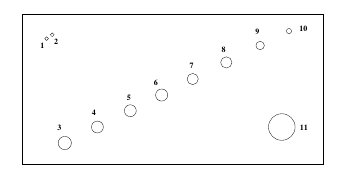
\includegraphics[width=0.2\textwidth]{pics/block.jpg}
\caption{\mbox{Acryllblock}}
\end{wrapfigure}
Anschließend soll mittels A-Scan die Abmessung eines Augemodells berechnet werden.

\begin{wrapfigure}[6]{r}{3.5cm}
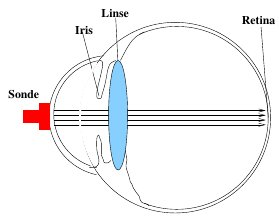
\includegraphics[width=0.2\textwidth]{pics/auge.jpg}
\caption{\mbox{Augenmodell}}
\label{pic_auge}
\end{wrapfigure}

Zunächst werden verschieden lange Acryllzylinder mittels Durchlaufverfahren beschallt. Aus der Laufzeit der Welle und der bekannten Abmessung des Zylinders wird so die Schallgeschwindigkeit im Acryll bestimmt.

Anschließend wird der Acryllblock mit den Fehlstellen untersucht. Hierzu verwendet man das Echo-Impuls-Verfahren auf beiden Seiten des Blockes um die genaue Lage und die Ausdehnung der Löcher zu finden.

Das Augenmodell wird ebenfalls mit dem Echo-Impulsverfahren untersucht. Gemessen werden sollen die Abstände: Hornhaut-Iris, -Linse und -Retina.


\section{Auswertung}
\subsection{Fehlerrechnung}
Da viele für die Auswertung notwendigen Größen fehlerbehaftet sind, ist es wichtig, den Einfluss dieser Fehler auf die ermittelten
Größen herauszufinden. Neben den, von den Messapparaturen verursachten Fehlern, dienen der Mittelwert
\begin{formel}[H]
\begin{equation}
 \bar{x} = \frac1N \sum_{i=1}^{N} x_i,
 \label{eq_mittel}
\end{equation}
\caption*{\small{$\bar{x}$ = Mittelwert, N = Anzahl der Messungen}}
\end{formel}

die Gaußsche Fehlerfortpflanzung

\begin{formel}[H]
\begin{equation}
\Delta G = \sqrt{\sum_{i=1}^{N}\left( \frac{\partial G}{\partial x_i}\cdot \Delta x_i\right)^2},
\label{gauss}
\end{equation}
\caption*{$x_i$ = Variable, $\Delta x_i$ = Fehler der Variable}
\end{formel}
und die Standardabweichung des Mittelwerts

\begin{equation}
 \bar s = \sqrt{\frac{1}{N(N-1)} \sum_{i}^{N} (x_i - \bar{x})^2}.
 \label{eq_standard}
\end{equation}

\subsection{Schallgeschwindigkeit in Acryl}
Um in Abschnitt \ref{sec_bohrung} die Abmessungen der Bohrungen in einem Acrylblock ermitteln zu können, ist die Bestimmung der Schallgeschwindigkeit 
in Acryl vonnöten. Hierzu werden das Impuls-Echo-Verfahren und das Durchschallungs-Verfahren genutzt. Zuvor werden die Höhen der verwandten
Acrylzylinder, sowie des -blocks mit einer Schieblehre ausgemessen, nach \eqref{eq_mittel} gemittelt und ihr Fehler entsprechend 
\eqref{eq_standard} bestimmt. Die Ergebnisse sind in Tabelle \ref{tab_masse} aufgeführt.

\begin{table}[H]
 \begin{tabular}{c|c|c|c|c}
  & Klein & Mittel & Groß & Block\\
  \hline
	&39,6&	80,5&	120,7&	77,3\\
Höhe 	&39,7&	80,4&	120,7&	77,6\\
in 	&39,7&	80,5&	120,6&	77,5\\
mm 	&39,7&	80,5&	120,5&	77,6\\
	&39,7&	80,5&	120,5&	77,7\\
	\hline
Mittelwert	&39,68$\pm$0,0004&	80,48$\pm$0,0004 &	120,6$\pm$0,002&	77,54$\pm$0,0046
 \end{tabular}
 \caption{Ausmaße verwandter Acrylkörper}
\label{tab_masse}
\end{table}

\subsubsection{Bestimmung mittels Impuls-Echo-Verfahren}
\label{sec_impulsecho}
In Tabelle \ref{tab_impulsecho} ist für die drei Zylinder die durch drei verschiedene Ultraschallsonden gemessene Laufzeit aufgeführt. Der
entstehende Fehler von $\Delta t$ = 0,1 $\mu$s wird vom Computerprogramm angegeben.

\begin{table}[H]
 \begin{tabular}{c|c|c|c}
 Ultraschallsonde & Klein & Mittel & Groß\\
 \hline
1 MHz (blau)&	30,6&	60,4&	89,7\\
2 MHz (rot)&	29,9&	59,7&	88,8\\
4 MHz (grün)&	29,4&	59,1&	88,5\\  
 \end{tabular}
\caption{Laufzeiten in $\mu$s bei den Acrylkörpern mit drei Sonden}
\label{tab_impulsecho}
\end{table}

Aufgrund der Anpassungsschicht der Ultraschallsonden, muss die Gleichung \eqref{eq_strecke} um den Laufzeitfehler $t_f$ modifiziert werden.
Aus der Differenz der Laufzeitstrecken $\delta s$ in \eqref{eq_laufzeitstrecke} lässt sich die Schallgeschwindigkeit in Acryl ohne 
Laufzeitfehler bestimmen. Die Gleichungen

\begin{align}
\label{eq_laufzeitfehler}
 s_i &= \frac12 c (t_i - t_f)\\
 \nonumber
 s_j &= \frac12 c (t_j - t_f)\\
 \delta s &= s_i - s_j = \frac12 c \cdot  \delta t = \frac12 c (t_i - t_j)
 \label{eq_laufzeitstrecke}
\end{align}
führen zur Schallgeschwindigkeit

\begin{align}
 c = 2\, \frac{\delta s}{\delta t}.
\end{align}
Ihr Fehler errechnet sich aus \eqref{gauss} zu

\begin{align}
 \Delta c = \sqrt{\left(\frac{\partial c}{\partial \delta s} \Delta s \right)^2 + \left(\frac{\partial c}{\partial \delta t} \Delta t \right)^2} = c\, \sqrt{\frac{\Delta s}{\delta s}^2 + \frac{\Delta t}{\delta t}^2}.
\end{align}
In Tabelle \ref{tab_schall} sind die Ergebnisse zur Schallgeschwindigkeit aufgeführt. 
\renewcommand{\arraystretch}{1.5}
\begin{table}[H]
 \begin{tabular}{c|c|c|c|c}
Sonde & Größe & Klein-Groß & Klein-Mittel & Mittel-Groß\\
\hline
&$\delta s$ in mm	&	80,92$\pm$0,002&	40,80$\pm$0,0005&	40,12$\pm$0,002\\
\hline
\hline
1 MHz &$\delta t$ in $\mu$s &59,1$\pm$0,1&	29,8$\pm$0,1&	29,3$\pm$0,1\\
&$c$ in km/s		&2,74$\pm$0,0046&	2,74$\pm$0,0092	&	2,74$\pm$,0093\\
\hline
2 MHz &$\delta t$ in $\mu$s &	58,9$\pm$0,1&	29,8$\pm$0,1&	29,1$\pm$0,1\\
&$c$ in km/s		&2,75$\pm$0,0047&	2,74$\pm$0,0092	&	2,76$\pm$,0095\\
\hline
4 MHz &$\delta t$ in $\mu$s &	59,1$\pm$0,1&	29,7$\pm$0,1&	29,4$\pm$0,1\\
&$c$ in km/s		&2,74$\pm$0,0046&	2,75$\pm$0,0093&	2,73$\pm$,0093\\
 \end{tabular}
\caption{Schallgeschwindigkeit $c$ in Acryl ermittelt durchs Impuls-Echo-Verfahren}
\label{tab_schall}
\end{table}
\renewcommand{\arraystretch}{1.0}
Aus den Werten ergibt sich für die Schallgeschwindigkeit in Acryl ein gemittelter Wert von

\begin{align}
 c = 2,742\pm0,003 \text{km/s}.
\end{align}

Der in Abschnitt \ref{sec_bohrung} benutzte Acrylblock wird mit der blauen Ultraschallsonde untersucht und das Augenmodell in Abschnitt 
\ref{sec_auge} mit der roten. Die dort ebenfalls auftretenden Laufzeitfehler $t_{f,i}$ können mit der ermittelten Schallgeschwindigkeit 
nach \eqref{eq_laufzeitfehler} errechnet werden. Das Ergebnis ist in Tabelle \ref{tab_laufzeitfehler} zu finden.

\begin{table}[H]
 \begin{tabular}{c|c|c|c|c}
Ultraschallsonde & Klein & Mittel & Groß & Mittelwert\\
 \hline
  $t_{f,blau}$ in $\mu$s &1,65$\pm$0,037	&1,69$\pm$0,035	&1,72$\pm$0,035 & 1,69$\pm$0,014 \\
  $t_{f,rot}$ in $\mu$s &0,95$\pm$0,025	&0,99$\pm$0,021	&0,82$\pm$0,017 & 0,92$\pm$0,010
 \end{tabular}
\caption{Laufzeitfehler der blauen Ultraschallsonde beim Impuls-Echo-Verfahren}
\label{tab_laufzeitfehler}
\end{table}

\subsubsection{Bestimmung mittels Durchschallungs-Verfahren}
\label{sec_durchschall}
In Tabelle \ref{tab_durchschall} sind die Laufzeiten nach dem Durchschallungs-Verfahren errechnet. Der Fehler $\Delta t$ = 0,1 $\mu$s
wird vom Computerprogramm angegeben.

\begin{table}[H]
 \begin{tabular}{c|c|c|c}
 Ultraschallsonde & Klein & Mittel & Groß\\
 \hline
1 MHz (blau) & 17,2&	32,1&	46,7\\
2 MHz (rot) &16,2&	30,9&	45,4\\
4 MHz (grün) &15,8	&30,5&	45,1  
 \end{tabular}
\caption{Laufzeiten in $\mu$s bei den Acrylkörpern mit drei Sonden}
\label{tab_durchschall}
\end{table}

Analog zu Abschnitt \ref{sec_impulsecho} wird die Schallgeschwindigkeit errechnet. Jedoch anders ist, dass die Laufzeitstrecke nun
nur noch halb so lang ist. Ergebnisse zur Schallgeschwindigkeit sind in der Tabellen
\ref{tab_schall_2} zu finden.
\renewcommand{\arraystretch}{1.5}
\begin{table}[H]
 \begin{tabular}{c|c|c|c|c}
Sonde & Größe & Klein-Groß & Klein-Mittel & Mittel-Groß\\
\hline
&$\delta s$ in mm	&	80,92$\pm$0,002&	40,80$\pm$0,0005&	40,12$\pm$0,002\\
\hline
\hline
1 MHz &$\delta t$ in $\mu$s &29,5$\pm$0,1&	14,9$\pm$0,1&	14,6$\pm$0,1\\
&$c$ in km/s		&2,74$\pm$0,009&	2,74$\pm$0,018	&	2,75$\pm$,019\\
\hline
2 MHz &$\delta t$ in $\mu$s &	29,2$\pm$0,1&	14,7$\pm$0,1&	14,5$\pm$0,1\\
&$c$ in km/s		&2,77$\pm$0,010&	2,78$\pm$0,019	&	2,77$\pm$,019\\
\hline
4 MHz &$\delta t$ in $\mu$s &	29,3$\pm$0,1&	14,7$\pm$0,1&	14,6$\pm$0,1\\
&$c$ in km/s		&2,76$\pm$0,009&	2,78$\pm$0,019	&	2,75$\pm$,019\\
 \end{tabular}
\caption{Schallgeschwindigkeit $c$ in Acryl ermittelt durchs Durchschallungs-Verfahren}
\label{tab_schall_2}
\end{table}
\renewcommand{\arraystretch}{1.0}
Daraus ergibt sich der Wert für $c$ zu

\begin{align}
 c = 2,759\pm0,005 \text{km/s}.
\end{align}

%\begin{table}[H]
% \begin{tabular}{c|c|c|c|c}
%Blaue Sonde & Klein & Mittel & Groß & Mittelwert\\
% \hline
%  $t_f$ in $\mu$s &2,82$\pm$0,088	&2,93$\pm$0,079	&2,98$\pm$0,078 & 1,69$\pm$0,041 \\
% \end{tabular}
%\caption{Laufzeitfehler der blauen Ultraschallsonde beim Durchschallungs-Verfahren}
%\label{tab_laufzeitfehler_2}
%\end{table}


\subsection{Untersuchung von Bohrungen in einem Acrylblock}
\label{sec_bohrung}
Der in Abbildung \ref{pic_block} gezeigte Acrylblock wird mit der blauen Ultraschallsonde (1 MHz) auf die Lage seiner Bohrungen
untersucht. In Tabelle \ref{tab_block} sind die Laufzeiten von oben und von unten aufgeführt, um somit Lage und Ausdehnung zu
ermitteln.

\begin{figure}[H]
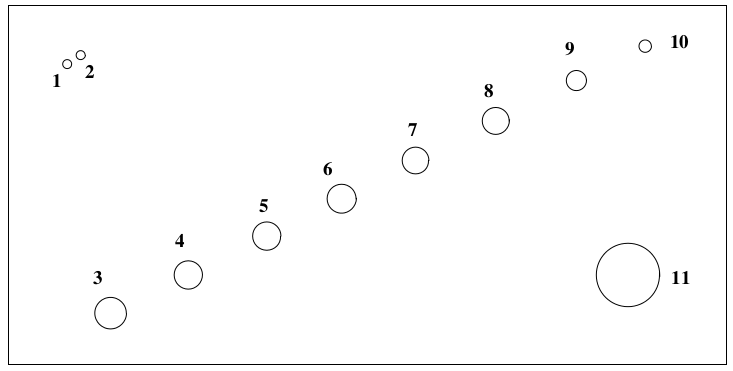
\includegraphics[width=0.7\textwidth]{pics/block.png}
\caption{Bohrungen im Acrylblock (aus Versuchsanleitung}
\label{pic_block} 
\end{figure}

Zur Errechnung von Lage und Durchmesser der Bohrungen werden folgende Gleichungen verwandten

\begin{align}
 s &= \frac12 c(t-t_f) \hspace{3cm} \text{(Abstand zur Sonde)}\\
 d &= h_{Block} - s_{oben} - s_{unten}. \hspace{1cm} \text{(Durchmesser der Bohrung)}
\end{align}

\begin{table}[H]
 \begin{tabular}{c|c|c|c|c|c}
 Nummer & $t_{unten}$ in $\mu$s& $t_{oben}$ in $\mu$s& $s_{unten}$ in mm& $s_{oben}$ in mm& $d$ in mm\\
 \hline
 \hline
1 &	44,7&	15,9&	58,96 $\pm$	0,15&	19,48$\pm$	0,14&	(-0,90)$\pm$	-0,007 \\
2&	45,7&	14,4&	60,33$\pm$	0,15&	17,43$\pm$	0,14&	(-0,22)$\pm$	-0,002\\
\hline
3&	11,1&	45,9&	12,90$\pm$	0,14&	60,61$\pm$	0,15&	4,03$\pm$	0,045\\
4&	17,2&	40,5&	21,26$\pm$	0,14&	53,20$\pm$	0,15&	3,07$\pm$	0,022\\
5&	23,6&	34,9&	30,04$\pm$	0,14&	45,53$\pm$	0,15&	1,97$\pm$	0,011\\
6&	29,9&	29,6&	38,67$\pm$	0,14&	38,26$\pm$	0,14&	0,60$\pm$	0,003\\
7&	35,8&	23,7&	46,76$\pm$	0,15&	30,17$\pm$	0,14&	0,60$\pm$	0,003\\
8&	41,6&	17,7&	54,71$\pm$	0,15&	21,95$\pm$	0,14&	0,88$\pm$	0,006\\
9&	47,4&	11,8&	62,66$\pm$	0,15&	13,86$\pm$	0,14&	1,02$\pm$	0,010\\
10&	n.D	&6,0&		n.D		&5,91$\pm$	0,14&	n.D	\\
\hline
11&	12,8&	41,3&	15,23$\pm$	0,14&	54,30$\pm$	0,15&	8,01$\pm$	0,076
 \end{tabular}
 \caption{Lage und Durchmesser der Bohrungen im Acrylblock}
 \label{tab_block}
\end{table}

Neben dem bisherigen Versuchsteil, der mit A-Scans durchgeführt wurde, bieten auch B-Scans eine Ermittlung der Körperinnenstruktur.
Für den Acrylblock ist in Abbildung \ref{pic_bscan} ein solcher B-Scan gezeigt, durchgeführt mit der roten Ultraschallsonden (2 MHz). 
Blau bedeutet hierbei keine Reflexion von Schallwellen, xrot entsprechend hohe Reflexionsrate.

\begin{figure}[H]
 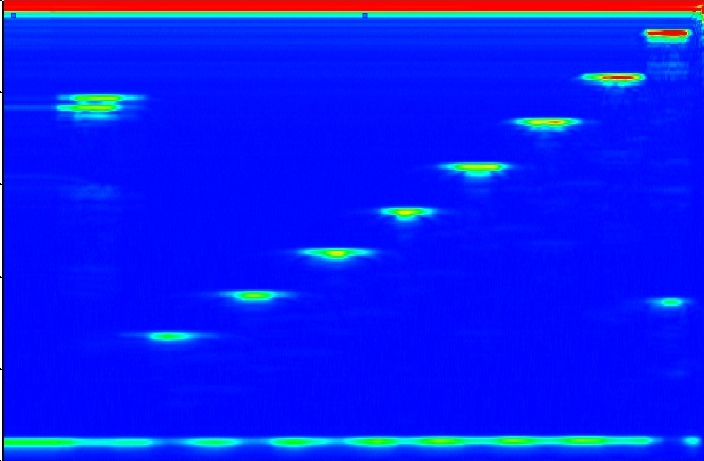
\includegraphics[width=1\textwidth]{pics/bscan-oben.jpg}
 \caption{B-Scan des Acrylkörpers}
 \label{pic_bscan}
\end{figure}

Anhand dieses Scans lassen sich ebenfalls, wenn auch sehr ungenau, Lage und Durchmesser der Bohrungen durch Ablesen bestimmen. Die
Ergebnisse sind in Tabelle \ref{tab_bscan} aufgeführt. Eine Fehlerrechnung erscheint hier wenig sinnvoll.

\begin{table}[H]
 \begin{tabular}{c|c|c}
Nummer & $s_{mittel}$ in mm & $d$ in mm\\
\hline
\hline
1	&19,39	&1,38 \\
2	&15,92	&1,38\\
\hline
3	&58,85	&1,45\\
4	&51,23	&1,59\\
5	&44,31	&2,15\\
6	&36,69	&2,15\\
7	&29,08	&2,08\\
8	&20,77	&2,35\\
9	&12,46	&2,56\\
10	&4,85	&1,32\\
\hline
11	&52,62	&1,66

 \end{tabular}
\caption{Aus B-Scan abgelesene Werte für Lage und Durchmesser}
\label{tab_bscan}
\end{table}

\subsection{Biometrische Untersuchung eines Augenmodells}
\label{sec_auge}
Ähnlich der Lagebestimmung von Bohrungen im Acrylblock, lässt sich in einem Augenmodell (siehe Abbildung \ref{pic_auge}) die innere
Struktur feststellen. Hierzu wurde die 2 MHz-Ultraschallsonde auf die Hornhaut gesetzt. Die gemessenen Zeiten sind in Tabelle \ref{tab_auge}
zu finden. Aufgrund der verschiedenen Schallgeschwindigkeiten im Auge werden die Messzeiten um den Laufzeitfehler reduziert und in ihre
Abschnitte eingeteilt, um danach zur Berechnung der Distanzen genutzt werden zu können.

\begin{table}[H]
\begin{tabular}{l|c|l|c}
Messbereich & $t$ in $\mu$s & Abschnitt & $t_{real}$ in $\mu$s \\
\hline
Hornhaut-Iris &	11,3	 &Hornhaut-Iris &	10,4\\
Hornhaut-Linse (außen) &	16,9	 &Iris-Linse (außen) &	6,5\\
Hornhaut-Linse (innen)	 &23,0	 &Linse (außen)-Linse (innen) &	6,1\\
Hornhaut-Retina &	72,9	 &Linse (innen)-Retina &	49,9
\end{tabular}
\caption{Laufzeiten in den Abschnitten des Augenmodells}
\label{tab_auge}
\end{table}

Mit den Schallgeschwindigkeiten
\begin{itemize}
 \item $c_{Hornhaut} = 1640^{[2]}$ m/s, \hspace{2cm}(Hornhaut-Iris)
 \item $c_{Linse} = 2500$ m/s, \hspace{2.6cm}(Linse)
 \item $c_{Glaskörper} = 1410$ m/s, \hspace{2cm}(Iris-Linse, Linse-Retina)
\end{itemize}
lassen sich nun die Distanzen (Maßstab berücksichtigt) nach \eqref{eq_strecke} errechnen. Die Ergebnisse sind in Tabelle 
\ref{tab_abmessung} aufgeführt.

\begin{table}[H]
 \begin{tabular}{l|c}
  Abschnitt & $s$ in mm\\
  \hline
Hornhaut-Iris	&2,84\\
Iris-Linse (außen)&	1,53\\
Linse (außen)-Linse (innen)&	2,54\\
Linse (innen)-Retina&	11,73
 \end{tabular}
\caption{Relativabstände von Augenbestandteilen}
\label{tab_abmessung}
\end{table}


\section{Diskussion}
Die ermittelten Werte für die Schallgeschwindigkeiten aus den Abschnitten \ref{sec_impulsecho} und \ref{sec_durchschall} werden 
nochmals genannt

\begin{align*}
  c = 2,742\pm0,003 \text{km/s},\\
  c = 2,759\pm0,005 \text{km/s}.
\end{align*}

Sie haben eine gute Übereinstimmung mit dem Literaturwert von 2730$^{[3]}$ km/s mit einer Abweichung von jeglich 0,4 \% bzw. 1,0\%. 

Die Lage der Löcher im Acrylblock ist gut bestimmt und passt gut mit der Abbildung \ref{pic_block} zusammen. Jedoch ergeben die Durchmesser
für die Störstellen Nummer 1 und 2 aufgrund des Vorzeichens keinen Sinn. Womöglich ist ihre Ausdehnung zu gering. Der B-Scan hat 
ebenfalls eine gute Übereinstimmung mit Abbildung \ref{pic_block}. Die Messung von Lage und Durchmesser hierbei ist durch Ablesefehler
sehr ungenau, jedoch ist eine etwaige Gleichheit mit den Ergebnissen aus den A-Scans feststellbar.

Über den inneren Aufbau des Auges lassen sich keine eindeutigen Aussagen treffen. Lediglich der Literaturwert zum Durchmesser von 
17-23$^{[4]}$ mm stimmt mit dem gemessenen Wert von $d_{Auge}$ = 18,6 mm überein. Die Relativabstände der inneren Bestandteile sind demnach
in einer sinnvollen Größenordnung.



\parskip 250pt
\Large{Literatur}\\\\
\large{[1] Versuchsanleitung - Grundlagen der Ultraschalltechnik}\\\\
\large{[2] Thannhäuser C.L. (2009), \textit{Messung der Hornhautdicke mittels Optischer Kohärenz-Tomographie (OCT)}, S.33}\\\\
\large{[3] Heine B. (2003), \textit{Werkstoffprüfung: Ermittlung von Werkstoffeigenschaften: mit 338 Bildern und zahlreichen Tabellen}, S.33}\\\\
\large{[4] Prof. Dr. Michelson G. (2000), \textit{Online Journal of Opthalmology}, \\URL: \href{http://www.onjoph.com/patinfo/funktion/zahlen.html}{www.onjoph.com/patinfo}}

% ========================================
%	Literaturverzeichnis
% ========================================

%\bibliographystyle{plainnat}			% Bibliographie-Style auswählen
%\bibliography{BIBDATEI}			% Literaturverzeichnis

% ========================================
%	Das Dokument endent
% ========================================

\end{document}
